%!TEX root =  ../main.tex

\chapterimage{Quantum_Plasma_Sphere} 
\mychapter{Sequences}{sss}

There are lists, adding up lists, and multiplying lists.

\newpage
\chapterminitoc

%									15 - 1
\newpage
\section{Sequences}
\subsection{Sequins}
\noindent\makebox[\textwidth]{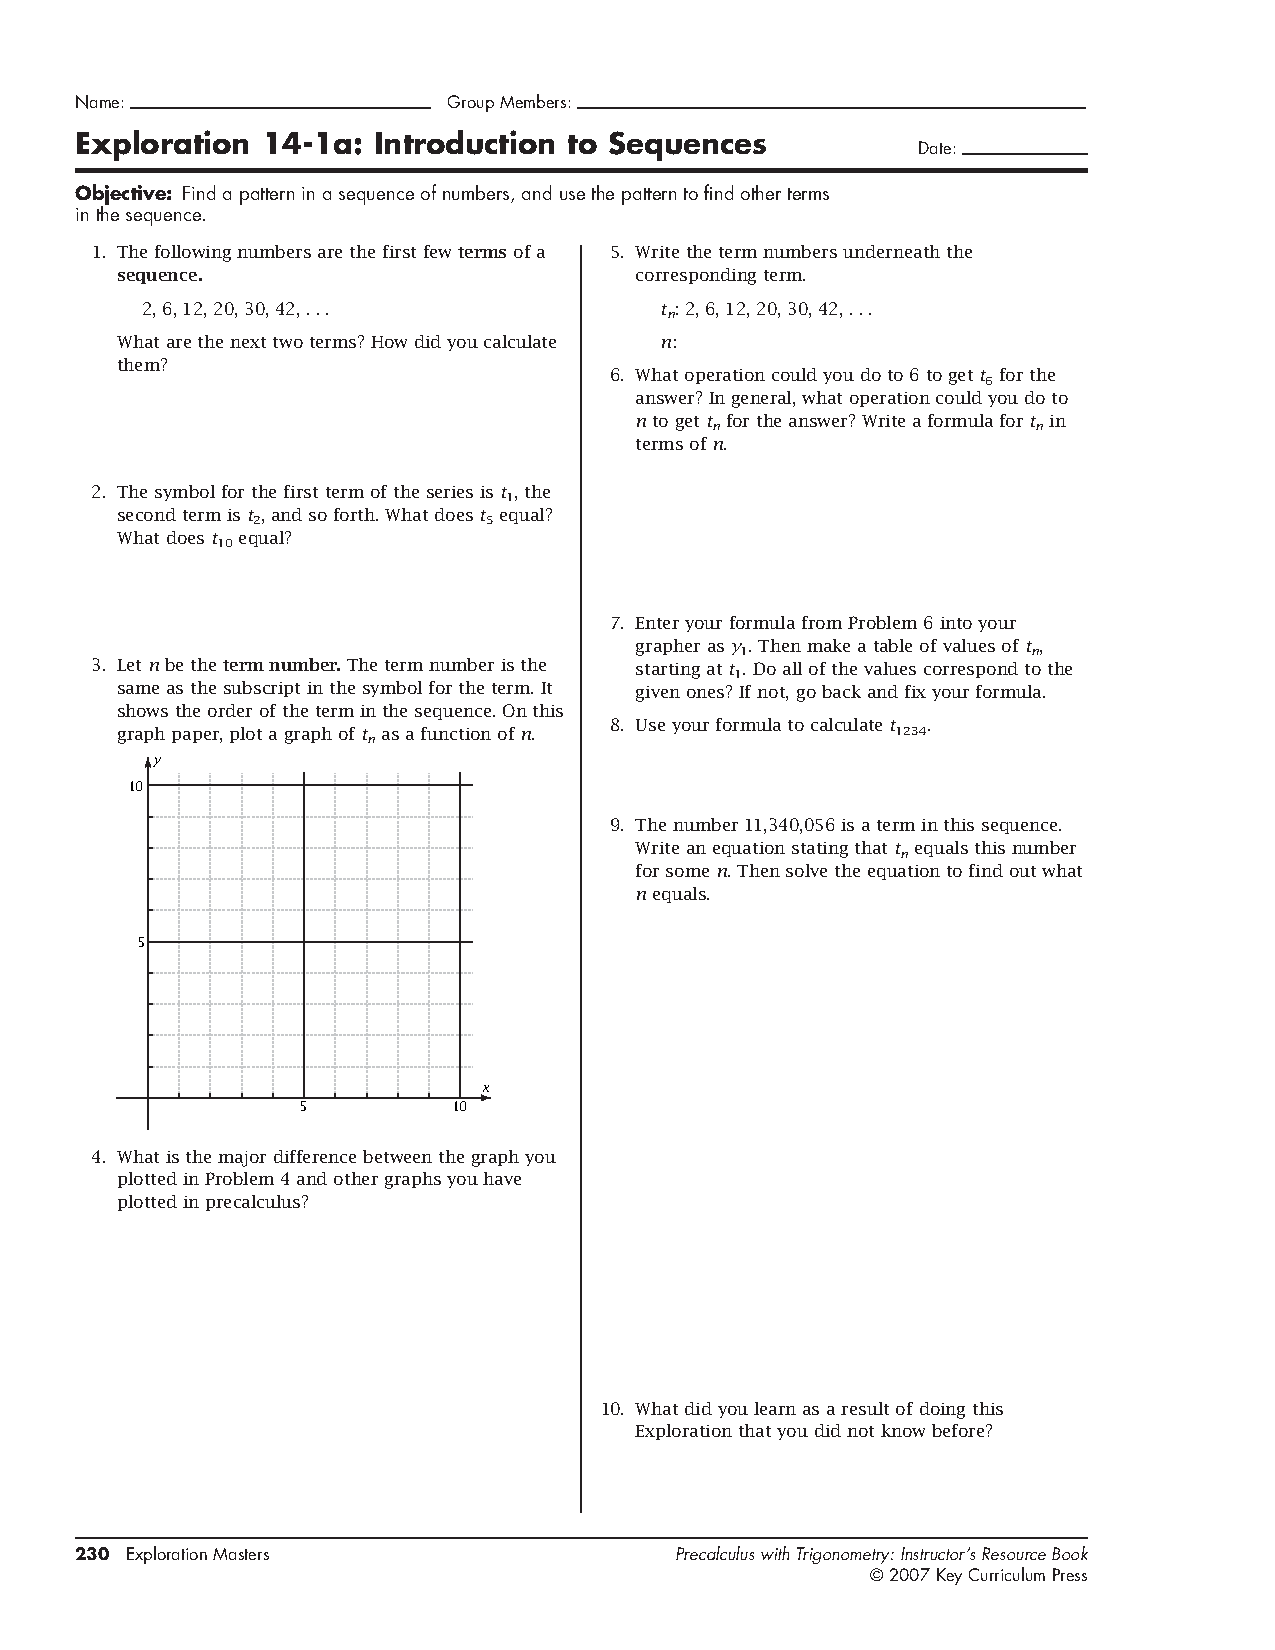
\includegraphics[width=\paperwidth]{ch15/1501p.pdf}}
\subsection{Recursion}
\subsection{Sequence Mode}
\subsection{Exercises}

%									15 - 2
\newpage
\section{Arithmetic and Geometric}
\noindent\makebox[\textwidth]{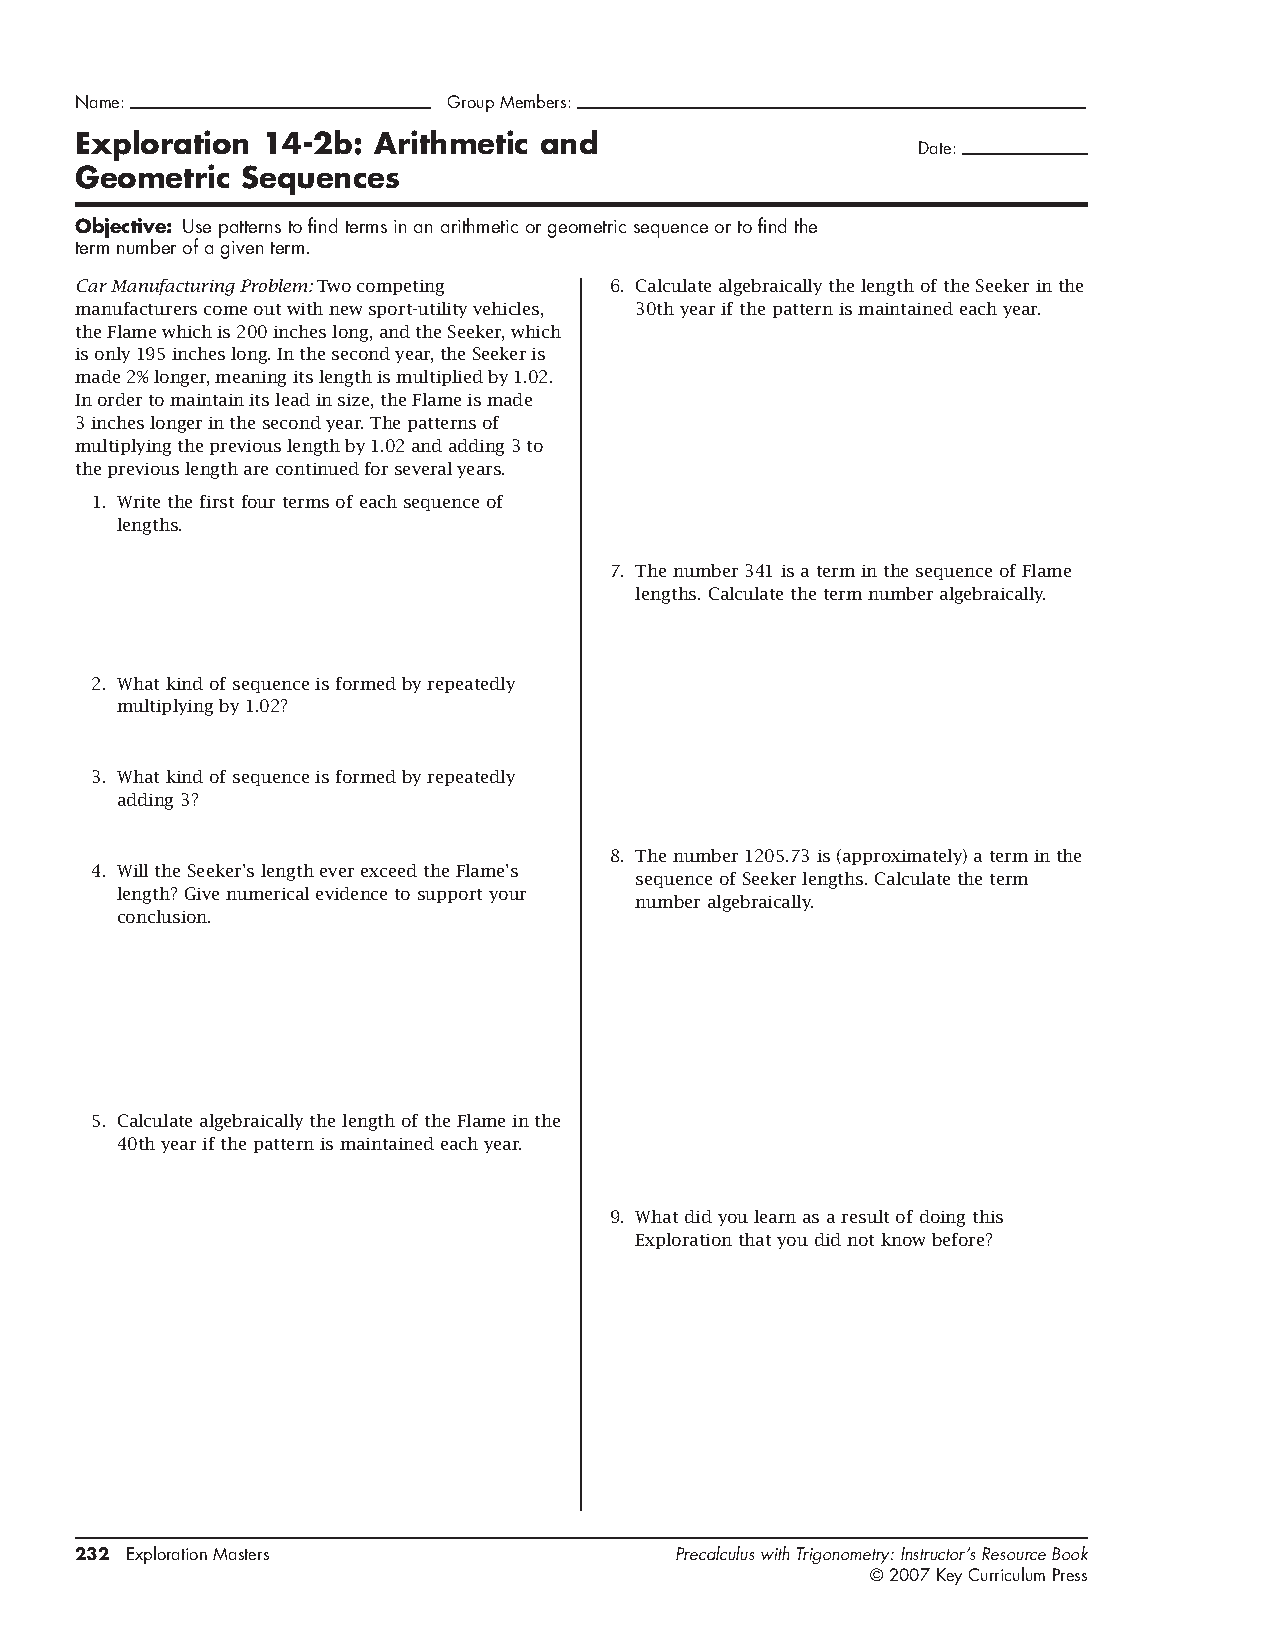
\includegraphics[width=\paperwidth]{ch15/1502p.pdf}}
\subsection{Repetition}
\subsection{Exercises}


%									15 - 3
\newpage
\section{Series and Partials}
\noindent\makebox[\textwidth]{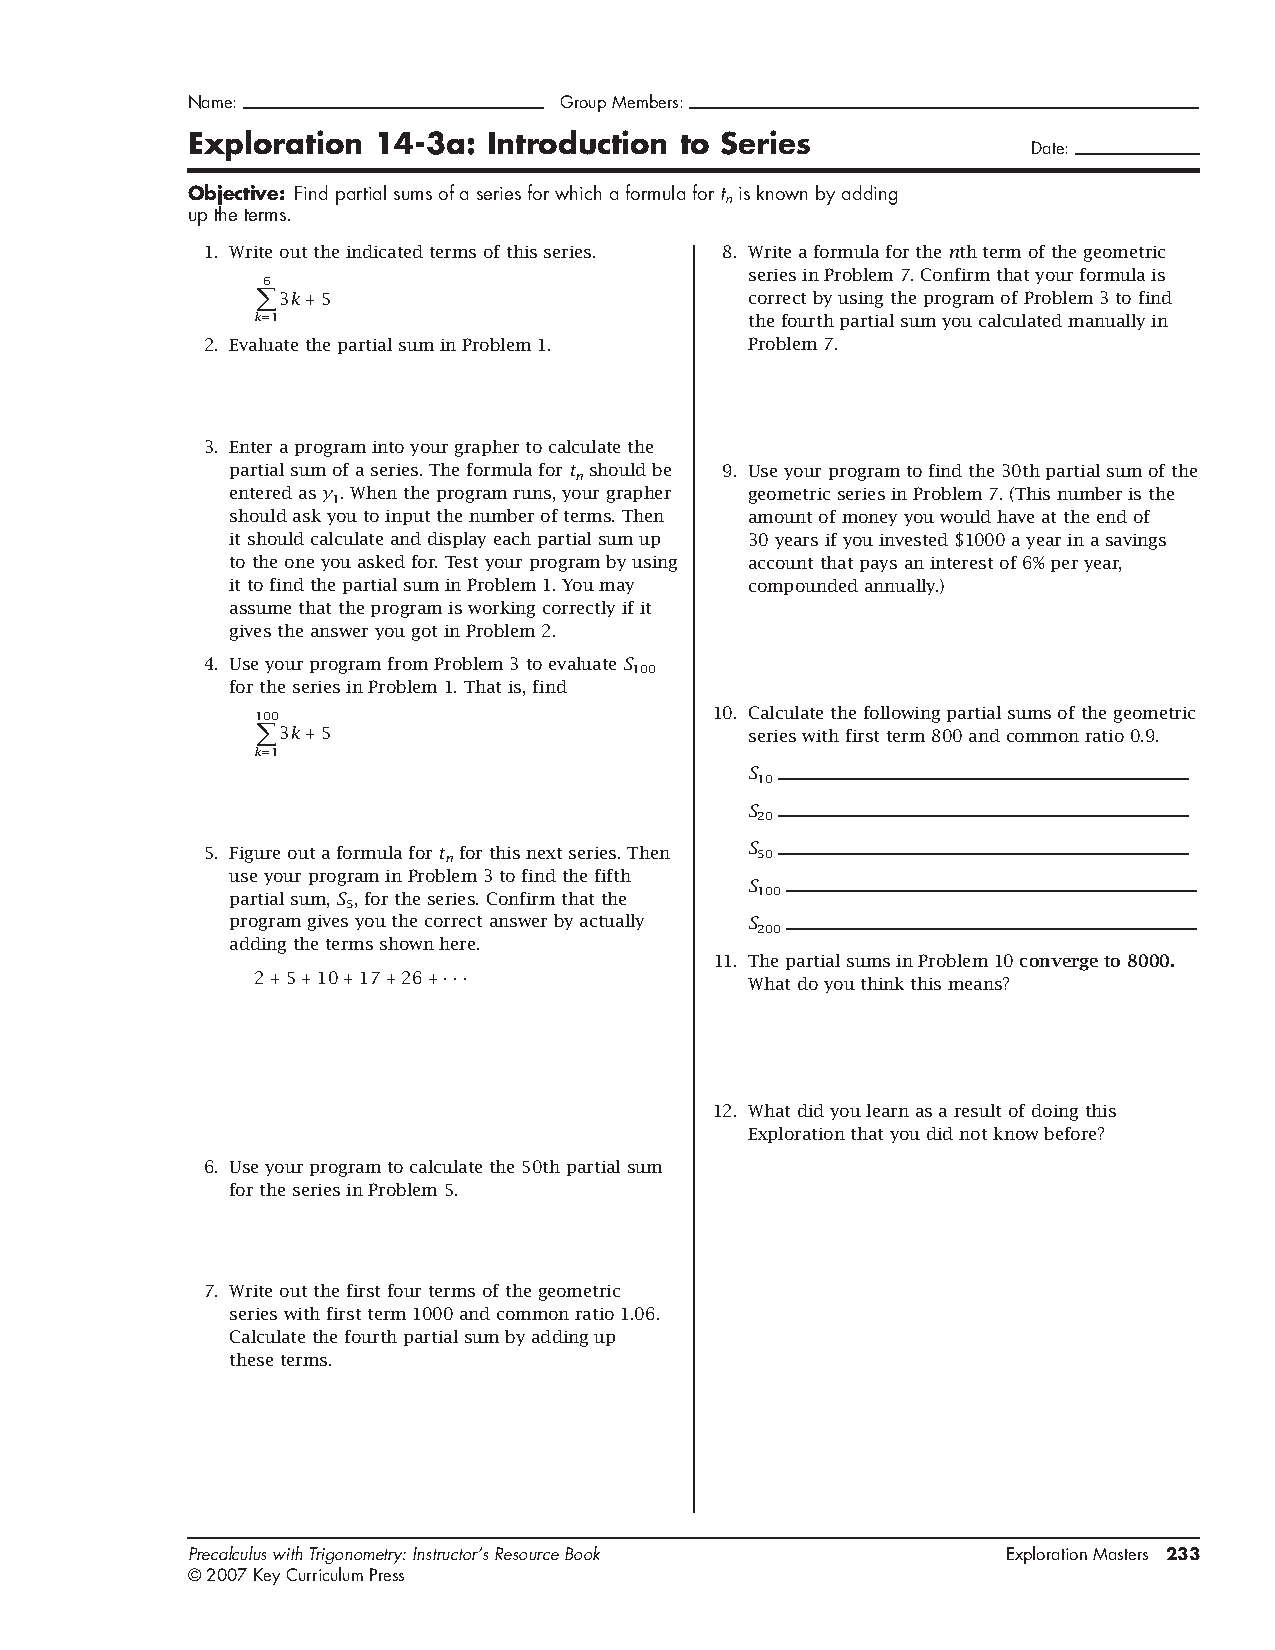
\includegraphics[width=\paperwidth]{ch15/1503p.pdf}}
\subsection{Exercises}

%									15 - 4
\newpage
\section{Infinite Series}
\noindent\makebox[\textwidth]{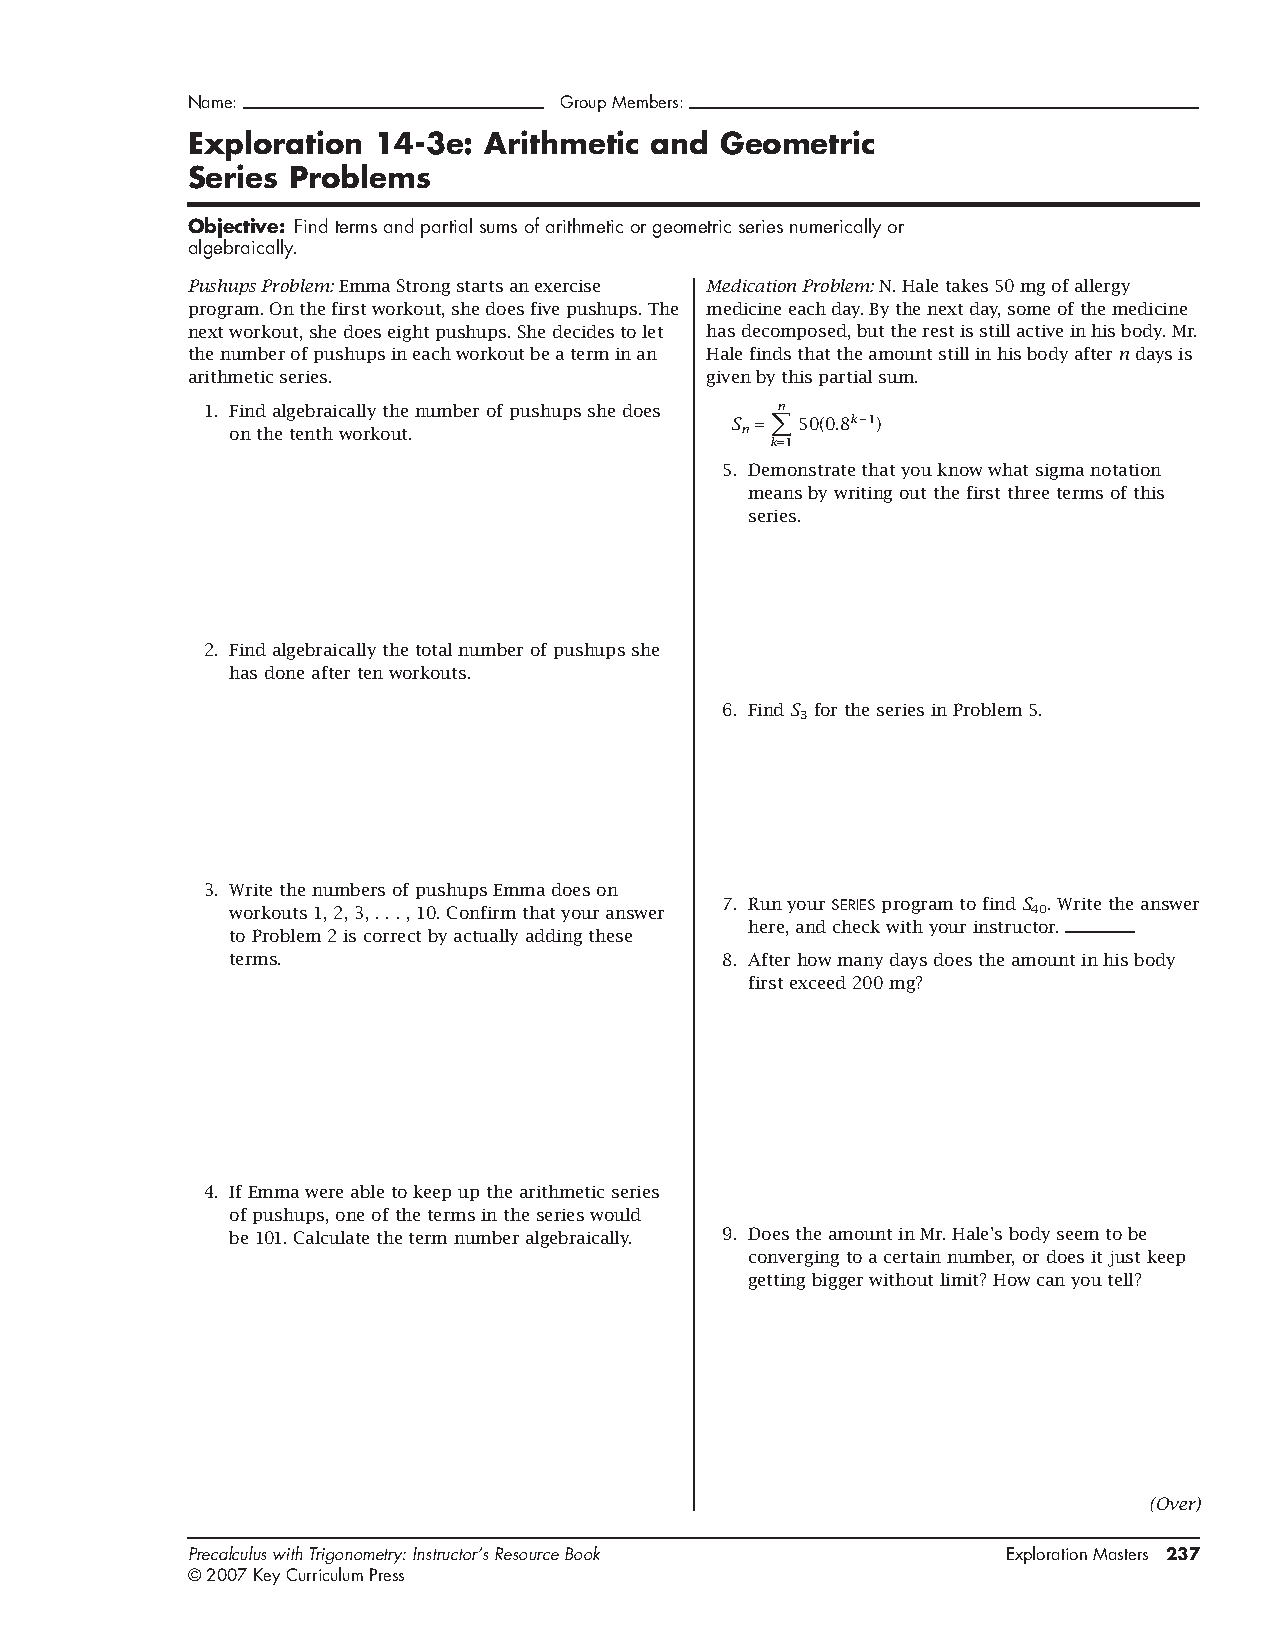
\includegraphics[width=\paperwidth]{ch15/1504p.pdf}}
\subsection{Formulae}
\subsection{Infinite}
% Save for 15
%intro to Zeta function $\zeta(s) = \frac{1}{1^s} + \frac{1}{2^s} + \frac{1}{3^s} + \dots$, 
%Partials, Cesàro summation, (of itself?)
%
\subsection{Exercises}

%									15 - 5
\newpage
\section{Pi Notations and Power Series}
\noindent\makebox[\textwidth]{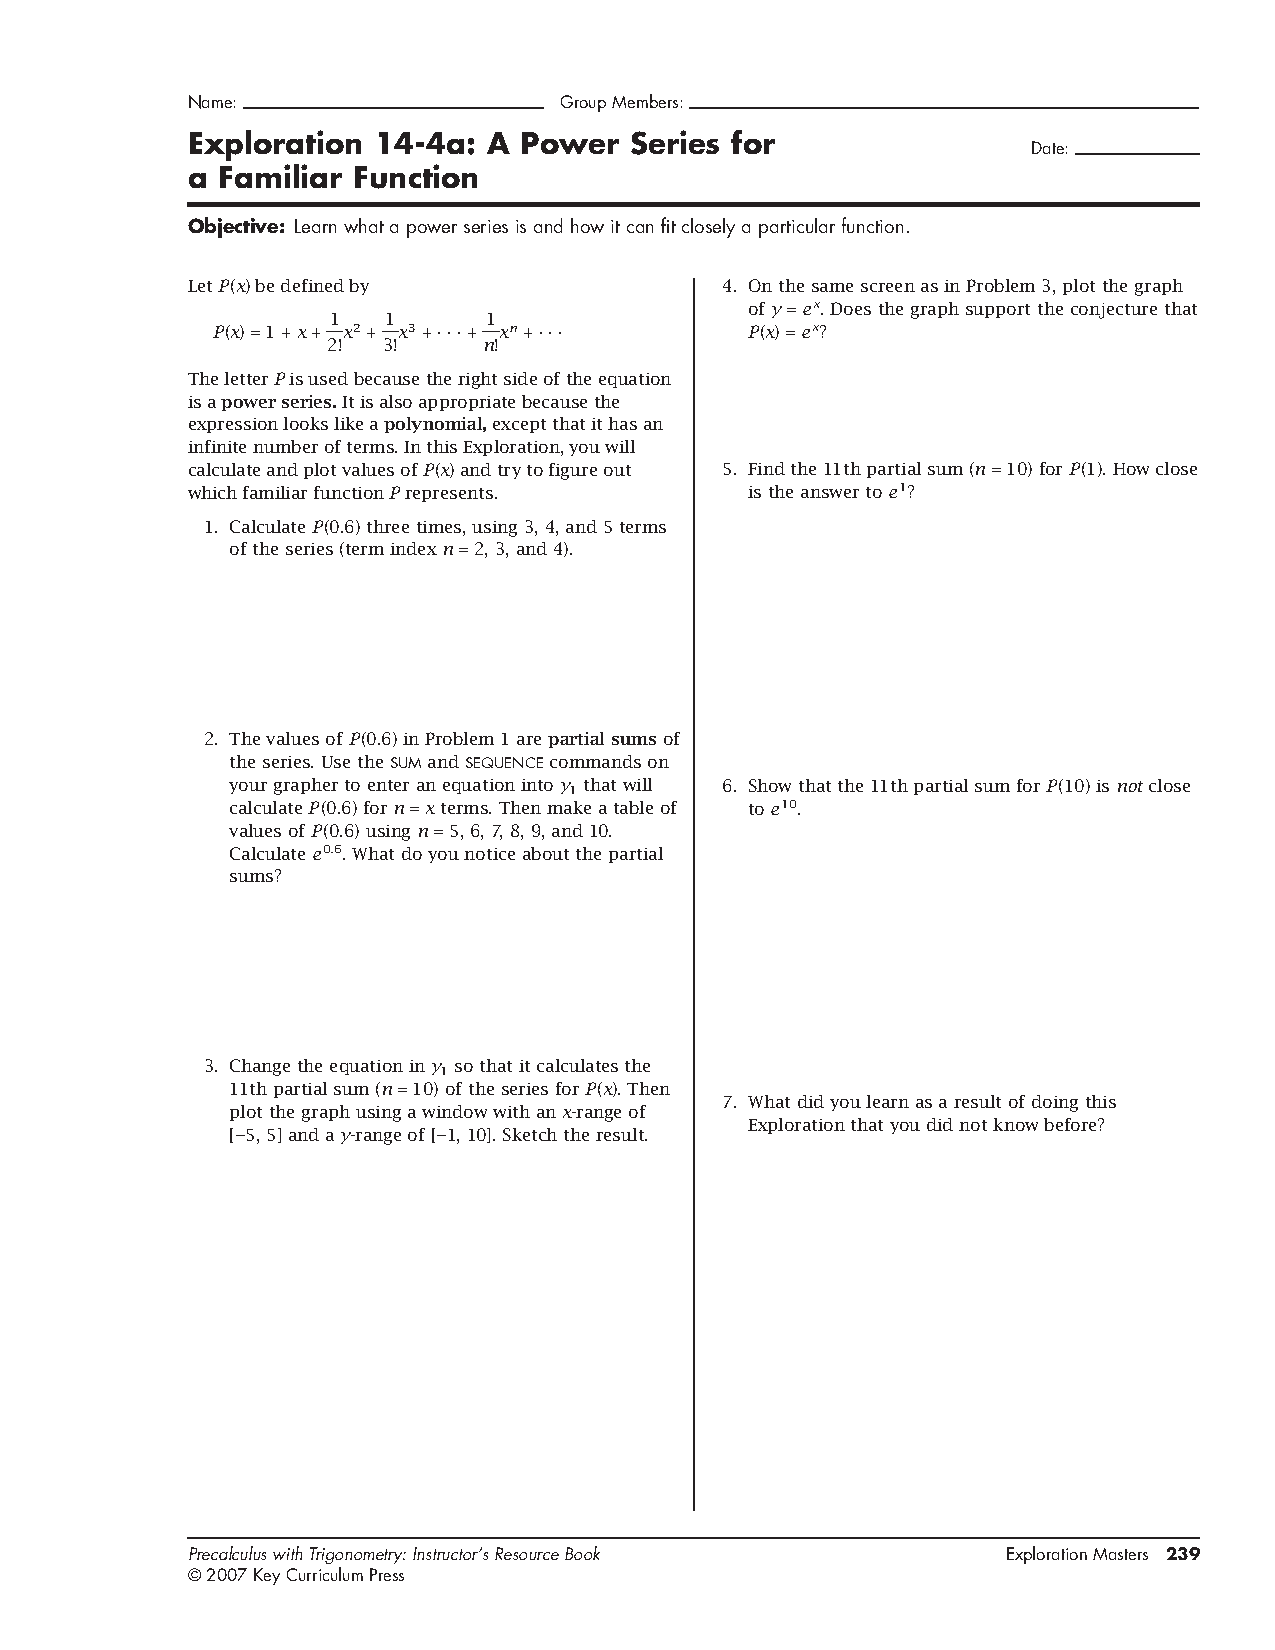
\includegraphics[width=\paperwidth]{ch15/1505p.pdf}}
\subsection{Exercises}


%									15 - 6
\section{Review}
\subsection{Chapter Review}
\subsection{Chapter Test}